\chapter{Introducción}
\label{chap:introduccion}

Este capítulo presenta las dificultades para sostener la facilitación de discusiones académicas asíncronas cuando aumenta la participación o el instructor debe atender varios hilos durante el mismo periodo. Después delimita el alcance, presenta los objetivos y las preguntas de investigación, describe el plan y el flujo de trabajo, y cierra con la estructura del resto del documento.

\section{Contexto}

Según el constructivismo social, el aprendizaje ocurre a través de la interacción, en la que los estudiantes construyen conocimiento discutiendo significados con otros estudiantes \parencite{WooReeves2007}. En educación superior, los debates son una de las técnicas que mejor aprovechan esta dinámica, porque aumentan el pensamiento crítico y el aprendizaje colaborativo \parencite{Brown2015}, dan voz a estudiantes más callados y crean un espacio de participación más equitativo que una clase netamente expositiva \parencite{BineyEkeyi2018,WooReeves2007}. Estas discusiones pueden tener lugar en el aula, donde un instructor guía el intercambio en tiempo real, o fuera de ella, a través de plataformas digitales. Fuera del aula, lo habitual es que el trabajo sea asíncrono, de modo que los participantes contribuyen en momentos distintos y sin necesidad de coincidir en el mismo lugar.

Las plataformas digitales que permiten este trabajo asíncrono han crecido significativamente en Europa durante los últimos años. En 2021, el 100\% de las instituciones del Espacio Europeo de Educación Superior ya usaba alguna forma de aprendizaje digital \parencite{GaebelEtAl2021}. Para 2025, el 75\% de las universidades utiliza el aprendizaje híbrido como modalidad principal y el 36\% ofrece al menos un programa de grado completamente en línea \parencite{GaebelEtAl2025}. Estas plataformas se conocen como sistemas de gestión del aprendizaje (\textit{Learning Management Systems}, LMS) y, dependiendo del tipo de institución, pueden constituir la modalidad principal del curso o complementar la educación presencial. Moodle, Canvas, Open edX y Coursera, por ejemplo, permiten organizar contenidos, actividades y foros de discusión en un mismo entorno, con cursos guiados por un instructor o desarrollados al ritmo del estudiante.

La pandemia de 2020 aceleró la adopción del aprendizaje digital. Durante los primeros cuatro meses de la crisis, varias instituciones reportaron más avances en digitalización que en los cuatro años anteriores \parencite{GaebelEtAl2021}. Como consecuencia, la interacción entre estudiantes pasó a ocurrir casi exclusivamente a través de herramientas digitales y los foros de discusión se consolidaron como uno de sus principales mecanismos en la educación en línea \parencite{Rovai2007,MasseyEtAl2019}.

En este contexto, los foros de discusión ofrecen formas de participación que resultan difíciles de mantener en un aula presencial, entre ellas la escala, la equidad de turnos y la flexibilidad horaria. Un estudio con más de 5.000 estudiantes en discusiones paralelas a través de Moodle muestra que permiten trabajar con un número de participantes que sería inmanejable en un aula tradicional \parencite{ZulfikarEtAl2019}. Además, cada estudiante dispone de más oportunidades para participar que en el formato presencial, donde el instructor puede concentrar hasta el 80\% del tiempo de habla \parencite{SullivanPratt1996}, ya que en los foros todos pueden contribuir con independencia de su ubicación o disponibilidad horaria \parencite{MasseyEtAl2019}. También permiten aplicar formas de evaluación basadas en la calidad de las aportaciones, con las que se puede medir el pensamiento crítico de manera más directa que mediante un examen tradicional \parencite{HoSwan2007,Rovai2007}.

Estas posibilidades han extendido el uso de los foros a contextos con escalas muy distintas, incluidos los cursos abiertos masivos en línea (MOOC, por sus siglas en inglés). A medida que aumentan el número de participantes y los hilos de discusión activos, también crece el trabajo necesario para facilitar las discusiones. Esta dificultad proporciona el punto de partida de la sección siguiente.

\section{Motivación}

La facilitación de las discusiones asíncronas recae principalmente sobre el instructor, que cumple un rol organizacional, uno intelectual y uno social \parencite{Abdous2011}. Cuando los asume de forma activa, la participación se distribuye de manera más equitativa entre estudiantes \parencite{AnEtAl2009}, el 79,3\% de las contribuciones alcanza pensamiento crítico profundo \parencite{LimEtAl2011} y la asignación de roles estructurados aumenta significativamente la construcción de conocimiento \parencite{DeWeverEtAl2010}. Sin embargo, este nivel de presencia tiene un límite práctico que la investigación sitúa entre 20 y 30 estudiantes por foro activo, y superarlo sobrecarga tanto a docentes como a estudiantes \parencite{Rovai2007}. Estudios de cursos de posgrado muestran que el 57\% de los comportamientos de presencia del instructor corresponde a la presencia social \parencite{RichardsonEtAl2015}, y la retroalimentación correctiva representó apenas el 4,9\% de las publicaciones a pesar de que los estudiantes la consideran esencial \parencite{BlignautTrollip2003}. Los facilitadores también informaron de que gestionar varias discusiones simultáneamente les impedía mantener la profundidad de su participación \parencite{Mansour2024}. El problema se acentúa en los MOOC, donde un solo curso puede concentrar miles de estudiantes \parencite{GuEtAl2021,YuEtAl2024maic}.

En los últimos años, plataformas como Coursera han integrado asistentes basados en grandes modelos de lenguaje (LLMs, por sus siglas en inglés) en más de 100 cursos para responder preguntas de estudiantes, con tiempos de respuesta un 47\% más rápidos que los tutores humanos \parencite{Coursera2024}, y edX alcanzó 1,2 millones de estudiantes en seis meses con laboratorios virtuales impulsados por inteligencia artificial (IA) \parencite{MarketGrowthReports2026}. Las revisiones disponibles documentan que estas aplicaciones se concentran principalmente en tutoría personalizada, generación de retroalimentación y asistencia al diseño curricular \parencite{ChuEtAl2025}. Sin embargo, la facilitación de discusiones grupales permanece menos explorada. El trabajo existente de procesamiento de lenguaje natural (NLP, por sus siglas en inglés) se concentra en tareas de clasificación, como la detección de toxicidad y el análisis de postura; la producción de intervenciones destinadas a mejorar la calidad de una discusión recibe menos atención \parencite{KorreEtAl2025}. Además, alrededor del 70\% de los estudios asignan a la IA la función de estructurar las condiciones de aprendizaje, mientras que la facilitación activa aparece con menor frecuencia \parencite{CasebourneEtAl2025}. Algunos trabajos abordan directamente la facilitación de discusiones, entre ellos un sistema de razonamiento por casos para generar sugerencias en foros en línea \parencite{GuEtAl2021}, y MAIC (\textit{Multi-Agent Intelligent Classroom}) escala la figura del instructor en entornos masivos usando múltiples agentes LLM \parencite{YuEtAl2024maic}.

\section{Alcance}

Este trabajo se centra en discusiones académicas asíncronas organizadas como hilos de texto, con independencia de la aplicación que las aloje. Esas discusiones pueden proceder de motores integrados en LMS, como Open edX, Moodle o Canvas, o de plataformas de conversación como Discourse. El objeto de estudio es la secuencia formada por el mensaje inicial, las respuestas, sus autores y sus marcas temporales, no una plataforma concreta.

La asincronía también delimita el problema técnico. El sistema no necesita responder mientras el estudiante escribe ni dentro de una conversación en tiempo real; puede analizar un hilo y preparar una intervención en segundo plano. Esta decisión reduce los requisitos de latencia y concurrencia y permite concentrar el trabajo en el proceso de facilitación: qué información observar, cuándo intervenir y qué tipo de respuesta proponer. Por tanto, el tiempo razonable de ejecución se interpreta según este contexto y no como el de una aplicación conversacional síncrona.

El artefacto recibe esos hilos mediante un contrato de entrada común, analiza su estado y decide si conviene generar una intervención. Su alcance funcional comprende la clasificación de la discusión, la selección de un rol y una técnica de facilitación, la generación de una respuesta y el registro de la ejecución para poder inspeccionarla. La activación automática desde cada plataforma y la publicación transparente en su interfaz nativa no se resolvieron de forma general.

Open edX se utilizó para construir y probar una fuente concreta de datos. Se implementaron un backend y puntos de comunicación capaces de recuperar hilos y alimentar el motor, junto con una prueba parcial de escritura. Esta prueba permitió estudiar el desacoplamiento respecto a la fuente, pero no constituye una integración end-to-end lista para uso docente. Completar la activación desde el flujo habitual del instructor y evitar que tenga que operar un panel adicional queda como trabajo futuro.

La facilitación continúa siendo responsabilidad del instructor. El sistema aborda decisiones que pueden describirse mediante evidencia observable, como si la conversación avanza, se estanca, se desvía o entra en conflicto, y qué tipo de apoyo podría corresponder. No modela rasgos psicológicos del docente ni evalúa o califica a los estudiantes.

El trabajo sigue de forma parcial el proceso de \textit{Design Science Research} (DSR) propuesto por Peffers et al. \parencite{PeffersEtAl2007}: identifica el problema, define objetivos, diseña y desarrolla el artefacto, lo demuestra con fuentes reproducibles y una conexión parcial con Open edX, y realiza una evaluación técnica preliminar. No se completó la evaluación de utilidad en un contexto educativo con estudiantes. La contribución se limita al motor, su demostración técnica y el marco de evaluación necesario para continuar ese ciclo.

\section{Objetivos}

El objetivo de este trabajo de fin de máster es diseñar e implementar un motor basado en LLMs y técnicas de context engineering para analizar y facilitar discusiones académicas asíncronas procedentes de distintas fuentes. El sistema debe usar el contenido del hilo, el contexto del curso y la literatura pedagógica para decidir si intervenir y producir una respuesta contextualizada.

Los objetivos específicos son los siguientes:

\begin{itemize}
  \item Diseñar e implementar un sistema de agentes basado en LLMs, organizado en etapas, capaz de producir intervenciones coherentes con el tema de la discusión y con continuidad conversacional, dentro de tiempos y consumo de recursos razonables.
  \item Definir e implementar una estrategia de context engineering fundamentada en la literatura, que integre el contenido del curso y literatura pedagógica sobre discusiones, con criterios de desempeño derivados de cómo un instructor facilita una discusión de forma efectiva.
  \item Definir un contrato de entrada independiente de la plataforma y comprobarlo mediante escenarios reproducibles, seis hilos históricos anonimizados conservados en el repositorio y una fuente parcial basada en Open edX.
  \item Evaluar el comportamiento del sistema en escenarios derivados de la literatura y en hilos importados, midiendo la clasificación del estado y la adecuación estimada de las intervenciones generadas.
\end{itemize}

\section{Plan de trabajo}

El trabajo se organiza en seis hitos que corresponden a las fases de un proyecto de I+D aplicado (tabla~\ref{tab:milestones}). Los dos primeros forman la fase exploratoria y los hitos 3 y 4 corresponden al diseño y la implementación; los dos últimos cubren la evaluación y la puesta en operación. La fase exploratoria delimita el problema de investigación, el alcance funcional y técnico y el enfoque metodológico. También reduce la incertidumbre técnica mediante la revisión del estado del arte, el estudio de las prácticas de un instructor efectivo y una serie de pruebas exploratorias (spikes) sobre el uso de LLMs para facilitar discusiones. De estas pruebas surge la estrategia de context engineering adoptada por el sistema.

La fase de diseño e implementación construye el motor en Python, define el contrato común para recibir hilos y desarrolla el panel con el que se lanzan e inspeccionan análisis. Open edX se usa como una de las fuentes para probar ese contrato, no como límite de la arquitectura. El hito 5 evalúa el sistema en escenarios reproducibles y en seis hilos históricos anonimizados conservados en el repositorio mediante clasificación automática y evaluación de las intervenciones. También documenta las limitaciones que deberán considerarse en una futura validación con estudiantes. Por último, el hito 6 despliega el artefacto en dos entornos de experimentación.

\begin{table}[h]
\centering
\small
\renewcommand{\arraystretch}{1.15}
\begin{tabularx}{\textwidth}{@{}Z{3.3cm}YZ{2.2cm}@{}}
\toprule
\textbf{Hito} & \textbf{Descripción} & \textbf{Se documenta en} \\
\midrule
1. Definición del problema & Formalización del problema, objetivos, requisitos y enfoque metodológico. & Cap.~\ref{chap:introduccion} \\
2. Investigación y exploración & Pruebas de concepto para reducir incertidumbre técnica antes del diseño. & Cap.~\ref{chap:estado-arte} \\
3. Implementación & Diseño e implementación del sistema a partir de los hallazgos del hito anterior. & \S\ref{sec:pipeline}--\ref{sec:prompts} \\
4. Fuentes de discusión & Contrato común de entrada y prueba parcial con Open edX. & \S\ref{sec:fuentes-discusion} \\
5. Control de calidad y feedback & Validación, recopilación de feedback y preparación de la documentación final. & Cap.~\ref{chap:resultados} \\
6. Despliegue e infraestructura & Puesta en operación de los entornos usados para los experimentos y la demostración técnica. & \S\ref{sec:entornos-ejecucion} \\
\bottomrule
\end{tabularx}
\caption{Hitos del proyecto, su descripción y dónde se documenta su resultado. El capítulo de desarrollo organiza el sistema por componente, así que varios hitos comparten sección.}
\label{tab:milestones}
\end{table}

La extensión de cinco a seis hitos se decidió durante la ejecución del proyecto, al comprobarse que los entornos disponibles condicionaban qué modelos y fuentes podían evaluarse. El capítulo de desarrollo organiza el sistema resultante por componente; la tabla anterior conecta cada hito con la sección donde se documenta su resultado.

La figura~\ref{fig:roadmap-github-project} complementa este resumen con la cronología registrada en GitHub Project. Las tareas iniciales de justificación, configuración y revisión de literatura precedieron a las pruebas de concepto. A partir de abril de 2026 se solaparon el diseño del modelo de intervención, la arquitectura multiagente, el repertorio de técnicas, la integración con Open edX y la infraestructura de evaluación. La captura muestra ese solapamiento y la relación de cada tarea con el issue donde se documentó.

\begin{landscape}
\begin{figure}[p]
\centering
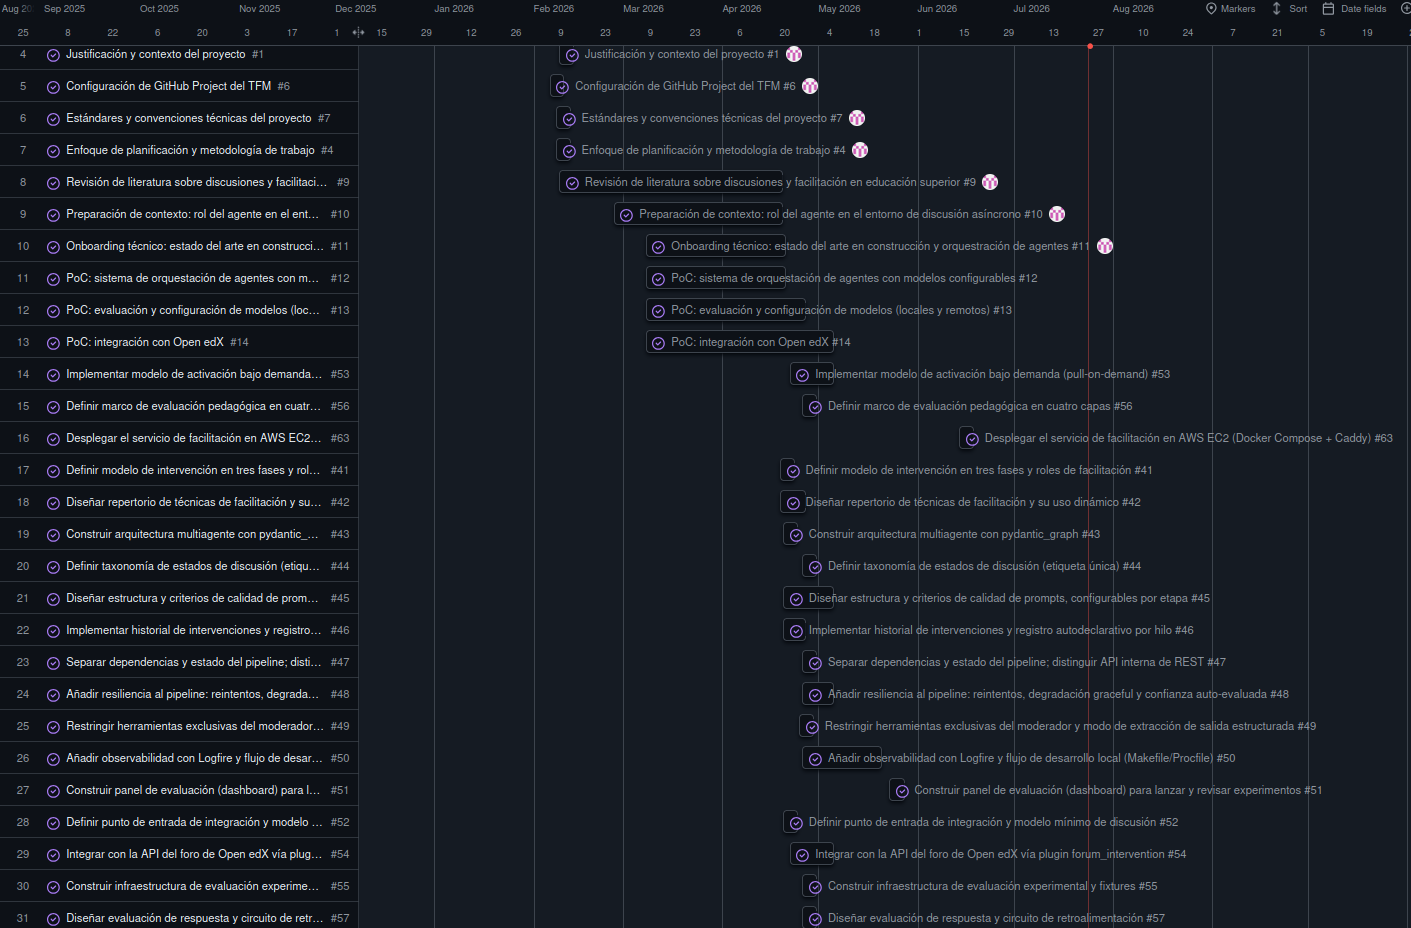
\includegraphics[width=\linewidth]{figures/roadmap-github-project.png}
\caption{Cronología del proyecto registrada en GitHub Project. Cada barra corresponde a una tarea vinculada con su issue; la vista refleja tanto la secuencia como el solapamiento del trabajo de investigación, implementación, integración y evaluación.}
\label{fig:roadmap-github-project}
\end{figure}
\end{landscape}

\section{Preguntas de investigación}

La investigación comenzó con preguntas exploratorias, antes de tomar ninguna decisión de diseño. El punto de partida fue la observación de que las discusiones asíncronas en plataformas educativas no producen el tipo de aprendizaje que sí ocurre en un aula presencial, y que no estaba claro por qué ni qué se podría hacer al respecto.

\subsection{Fase exploratoria}

Las primeras preguntas apuntaban a entender esa dinámica:

\begin{itemize}
  \item ¿Qué ocurre en un aula presencial que no ocurre en una discusión asíncrona? ¿Por qué la dinámica social del aprendizaje no se traslada a los foros de texto?
  \item ¿Qué hace a un facilitador efectivo? ¿Qué acciones concretas produce un instructor cuando interviene en una discusión?
  \item ¿Cómo se ve el proceso de intervención desde dentro? ¿Qué información necesita un facilitador para tomar una decisión?
  \item ¿Es posible hacer ese proceso observable y controlable, o es opaco por naturaleza?
\end{itemize}

Estas preguntas guiaron la revisión de la literatura y la exploración técnica inicial. La respuesta a la cuarta pregunta, en particular, determinó la dirección del diseño, puesto que si el proceso de intervención puede describirse como un conjunto de condiciones observables más una acción correspondiente, puede implementarse como un pipeline; si no puede, la automatización no es viable. La evidencia de los sistemas de tutoría inteligente \parencite{VanLehn2011} y la literatura sobre roles de facilitación \parencite{PilkingtonWalker2003} sugirió que sí es posible, dentro de límites.

\subsection{Fase de diseño}

Una vez delimitado el problema, las preguntas se volvieron más concretas:

\begin{itemize}
  \item ¿Cómo pueden operacionalizarse los roles de facilitación como agentes LLM en un pipeline de análisis de discusiones?
  \item ¿Qué criterios permiten detectar automáticamente el estado de una discusión para determinar si y cuándo intervenir?
  \item ¿Qué criterios permiten evaluar si una intervención generada por IA es pedagógicamente adecuada?
  \item ¿Puede el motor recibir discusiones de una plataforma educativa sin acoplar el pipeline a su modelo de datos?
\end{itemize}

Estas preguntas estructuran el capítulo de desarrollo, ya que cada una corresponde a un componente del sistema o a una decisión de diseño documentada.

\section{Flujo de trabajo}

El proyecto usa un flujo de trabajo de I+D inspirado en prácticas ágiles, con kanban como herramienta de seguimiento pero sin sprints fijos. La incertidumbre propia de la investigación no se ajusta bien a iteraciones de duración predeterminada, algunas preguntas se resuelven en días y otras requieren semanas de exploración antes de poder tomar una decisión.

En la práctica, el trabajo se organiza en ciclos de descubrimiento, de forma que los hallazgos de cada fase informan la siguiente. Las herramientas principales son los issues, el tablero del proyecto y los Architecture Decision Records (ADRs), disponibles en el \href{https://github.com/magrimal/tfm-2026-discussion-moderation}{repositorio del proyecto}. Los \textbf{issues} recogen lo que debe explorarse o implementarse y proporcionan contexto suficiente para retomar el trabajo más adelante. El \textbf{tablero} muestra el estado del trabajo sin fijar sprints artificiales. Los \textbf{ADRs} registran las decisiones de diseño significativas, su razonamiento y las alternativas descartadas, por lo que funcionan como memoria del proyecto. Los \textbf{hitos} delimitan las fases; cada fase termina cuando se responden las preguntas que la definen, no cuando expira un plazo. Se prioriza el enlace al tablero sobre una captura, porque su contenido cambia durante el proyecto y la imagen quedaría desactualizada.

En esta memoria solo se reportan decisiones de diseño respaldadas por evidencia trazable en resultados, tablas, figuras o ADRs del proyecto. Antes de comprometerse con una implementación, cada área de incertidumbre técnica se aborda mediante un spike o prueba de concepto, sin calidad de producción, cuyo objetivo es reducir incertidumbre y documentar hallazgos, no entregar código mantenible.

\subsection{Uso de asistentes de IA en la implementación}

La implementación técnica se realizó con apoyo de asistentes de programación basados en LLM, en particular Claude y Codex. Se usaron para generar borradores de código y documentación, explorar alternativas, localizar inconsistencias y proponer pruebas. El trabajo siguió un ciclo iterativo de propuesta, revisión, prueba y corrección.

La autora definió el problema, aceptó o rechazó las propuestas y asumió la responsabilidad sobre las decisiones, los experimentos y el texto final. No se calculó un porcentaje de código humano o generado por IA, los cambios pasaron por varias iteraciones y el historial de Git no permite atribuir de forma fiable cada línea a una única fuente.

\section{Estructura del documento}

El documento se organiza en siete capítulos. El capítulo~\ref{chap:introduccion} presenta el problema, delimita el alcance y recoge los objetivos, las preguntas de investigación y el plan de trabajo; el capítulo~\ref{chap:introduction-en} ofrece su versión en inglés. El capítulo~\ref{chap:estado-arte} revisa la literatura sobre facilitación y los sistemas de IA que abordan partes del problema. El capítulo~\ref{chap:desarrollo} presenta la experiencia de uso del panel y explica el pipeline, sus decisiones de intervención, las fuentes de datos y los entornos de despliegue. El capítulo~\ref{chap:resultados} documenta los experimentos y las intervenciones generadas. Por último, el capítulo~\ref{chap:conclusiones} recoge las conclusiones, las limitaciones y el trabajo futuro, y el capítulo~\ref{chap:conclusions-en} presenta su versión en inglés.
